\section*{Question 1}
\emph{Investigate the stability and accuracy of the four schemes in terms of the Courant-Friedrichs-Lewy (CFL) numbers $\lambda = c \tfrac{dt}{dx}$ and $\mu = \nu \tfrac{dt}{{dx}^2}$. In particular use numerical experimentation and/or von Neumann stability analysis to determine stability boundaries.}
%
%\begin{figure}[!ht]
%\centering
%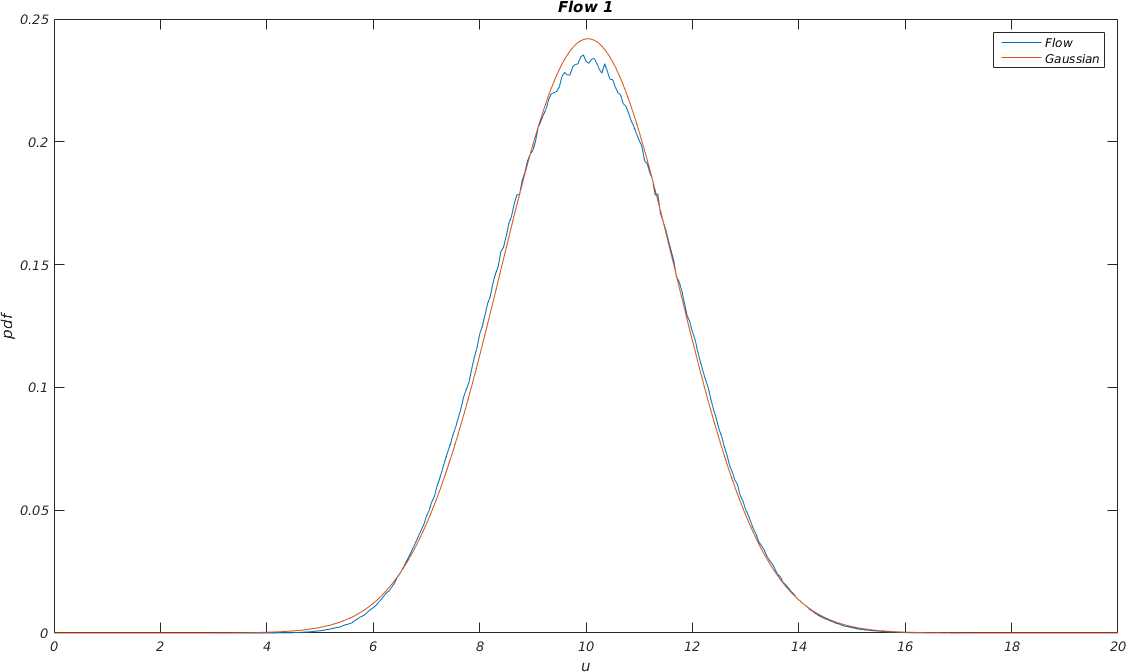
\includegraphics[scale=0.4]{./TEXT/pdf1.png}
%\caption{The Probability Density function for \emph{flow 1}}
%\label{pdf1}
%\end{figure}
%
%
%\begin{table}[ht]
%\caption{Comparison of the first four moments for the two flows.}
%\label{tbl1}
%\centering
%\begin{tabular}{l|c|c}
%& Flow 1 & Flow 2 \\
%\hline
%1\su{st} Moment: Mean & $10.04$ & $10.04$ \\
%\hline
%2\su{nd} Moment:Variance & $2.72$ & $2.72$ \\
%\hline
%3\su{rd} Moment:Skewness & $0.05$ & $0.05$\\
%\hline
%4\su{th} Moment:Kurtosis & $2.78$ & $2.78$ \\
%\hline
%\end{tabular}
%\end{table}
%
